\chapter{Writing extendable program (plug-ins, modular)}

One important functionality of writing an application is its extendibility. In
particular, it allows users to write a new module and add that to the existing
program easily.

A program can provide extensibility via C API or shared library modules.
To load a shared library module, we use \verb!dlopen()!
(Sect.\ref{sec:dynamic-load-library}).

\url{http://eli.thegreenplace.net/2012/08/07/fundamental-concepts-of-plugin-infrastructures}


\section{Breaking the chain of library dependency}

Because of the backward compatibility requirements of libc and Linux kernel, a
program/library compiled on an older version of Linux kernel should be able to
run on a machine with newer Linux kernel.

SUGGESTION: Compile the code on an old-enough Linux kernel, e.g. 2.6.9, and
distribute this code, which we hope that the systems with newer libraries can
run it. 
\begin{itemize}
  \item The problem is, the bundled gcc with this Linux kernel version, gcc
3.4.6 is quite old, and thus it cannot be used to compile the code if it is
using newer features, or it cannot be used to load the shared library if the
library uses the newer C++ features.

Example: the program use an extension in the form of shared library
\verb!customer_extension_module.so!.
\begin{verbatim}
$> ./myapp  

./myapp: libs/libstdc++.so.6: version `GLIBCXX_3.4.15` not found ( required by customer_extension_module.so )
\end{verbatim}  

SOLUTION: We ship the new \verb!libstdc++.so.6! built by the newest release gcc (e.g. 4.8.2)
on the old-enough Linux kernel. There are two steps: (1) compile gcc 4.8.2 from source 
on the old-enough Linux kernel, (2) using the compiled gcc 4.8.2 to compile the libstdc++ source
on the old-enough Linux kernel.
\begin{itemize}
  \item Step 1

\begin{verbatim}
  // only use libc++ library
~/gcc-build$> ../gcc-4.8.2/configure -disable-multilib -enable-languages=c,c++

  // do not replace the current gcc version (e.g. 3.4.6)
  // so put the new compiled gcc into a different folder
~/gcc-build$> make DESTDIR=/home/joe/gcc-output-tree install  
\end{verbatim}

This a set of shared libraries will load on platforms at least as old as the one
you're on, and \textcolor{red}{because of the backwards compatibility
requirements of libc and the Linux kernel}, should work on the most recent OS
distributions.

  \item Step 2: Build your application with this compiler, using the rpath
  technique to ensure it depends on the libraries you will ship
  
\end{itemize}
\end{itemize}

\section{Objective-C: NSBundles}


\section{C++: Boost.Extension, Pluma, DynObj, FxEngine}

The Boost.Extension was made to ease the development of plugins and similar
extensions to software using shared libraries. Classes, functions and data can be made available from shared libraries and loaded by the application.
However, for Boost.Extension, there is currently no support for C++0X, as it is
not easy to port it using the new 
\url{http://blog.redshoelace.com/2014/01/c0x.html}

\url{http://stackoverflow.com/questions/19474053/deciding-on-a-language-framework-for-a-modular-opencv-application}

\section{C: C-Pluff framework}


\begin{figure}[hbt]
  \centerline{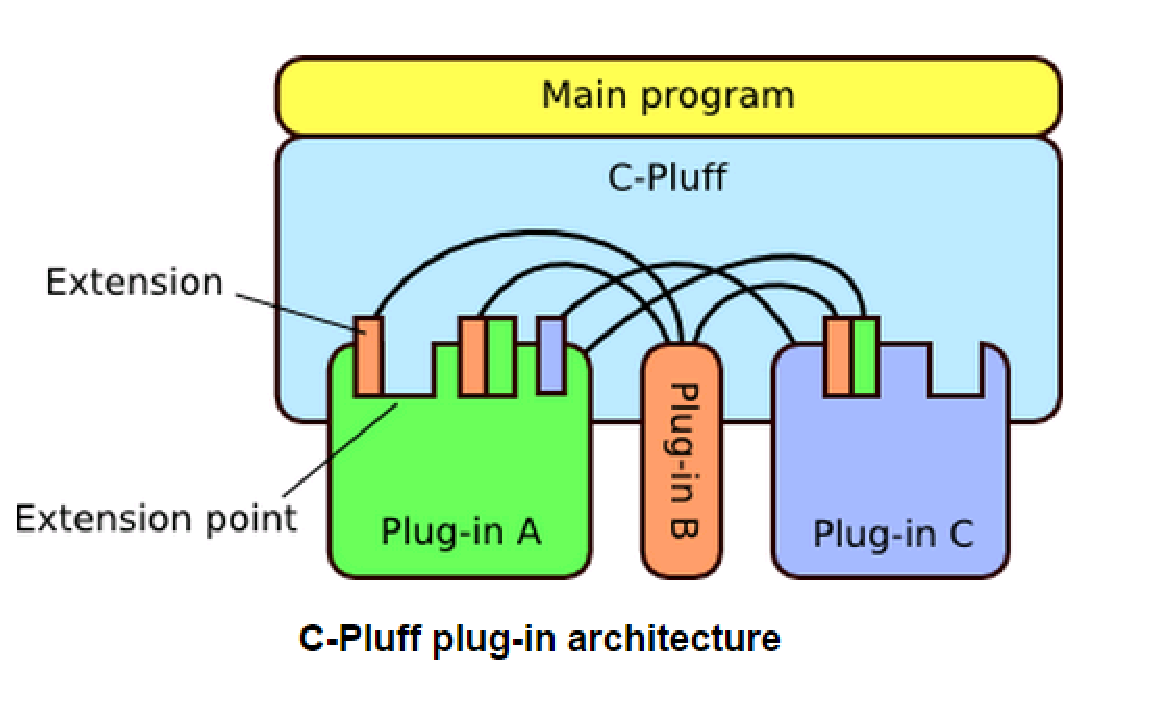
\includegraphics[height=5cm,
    angle=0]{./images/C-pluff_framework.eps}}
\caption{The main program: initialize and settup the plug-in environment.
Plug-ins integrate with each other by providing extension points and extensions.
An extension point is a point into which other plug-ins can attach extensions.}
\label{fig:C-pluff_framework}
\end{figure}

\url{http://www.c-pluff.org/reference/c-api/architecture.html}


\section{Case-study: valgrind 'core' + 'plug-ins'}


Valgrind (Sect.\ref{sec:valgrind}) is a powerful tool with 2 components:
\begin{itemize}
  \item  core: a common low-level infrastructure to support program
  instrumentation, including the JIT compiler, low-level memory manager, signal handling and a scheduler (for pthreads).
  
  The core leaves certain operations undefined, which must be filled by tools
  
  \item plug-ins: a set of tools that developed by users, and must implement
  the required list of functions for the core to use.
  
  Minimum set of functions
\begin{verbatim}
pre_clo_init()
post_clo_init()
instrument()
fini()
\end{verbatim}
\url{http://www.valgrind.org/docs/manual/writing-tools.html}
  
  The core/tool interface is not fixed. It's pretty stable these days, but it
  does change.
  
  A plug-in can also call certain functions to indicate to the core that they
  would like to use certain services, or be notified when certain interesting events
  occur. But the core takes care of all the hard work.
  
\end{itemize}

Once a plug-in is completed, it must be compiled and linked against Valgrind
core to become a complete Valgrind tool, which can be used by Valgrind via the
\verb!-tool! option to select it.

\subsection{Writing tools}


HINTS: 
From Valgrind source, the files \verb!include/pub_tool_*.h! contain all the
types, macros, functions, etc. that a tool should (hopefully) need, and are the
only .h files a tool should need to \verb!#include!.

Valgrind provides an implementation of a reasonable subset of the C library,
details of which are in \verb!pub_tool_libc*.h!



\section{Case-study: Wirebrush4SPAM}


\url{http://www.researchgate.net/profile/David_Ruano_Ordas/publication/243464849_Wirebrush4SPAM_a_novel_framework_for_improving_efficiency_on_spam_filtering_services/links/0046351d180f499daf000000.pdf}